\scanpage{571}
\mspage{290}

plus près les variétés modulaires congruentielles
$M_{1,1}[3]$ et $M_{1,1}[5]$, correspondant à des
groupes modulaires ``géométriques'' :
\[
\unsure{(}\quad
\left\{
\begin{array}{l}
S\Gamma'_3 = \underbrace{\mathrm{Sl}(2,\mathbb F_3)}_{\substack{\text{ordre }4.3.2\\=24}}/\mathord{\pm}1
\quad \text{d'ordre }12\;\underset{\unsure{\deleted{\unsure{\infty}}}}{\phantom{a}}
\subset \underbrace{\mathrm{GP}(1,\mathbb F_3)}_{\text{ordre }24}\simeq\mathfrak S_4
\\[1.5em]
\unsure{\inserted{\text{en fait, on doit avoir } S\Gamma'_4\simeq A_4}}
\\[1.5em]
S\Gamma'_5 = \underbrace{\mathrm{Sl}(2,\mathbb F_5)}_{\substack{\text{ordre }6.5.4\\=120}}/\mathord{\pm}1
\quad \text{d'ordre }60
\subset \underbrace{\mathrm{GP}(1,\mathbb F_5)}_{\text{ordre }120}\simeq\text{groupe du \uline{bi}icosaèdre}
\end{array}
\right.
\tag{74}
\]

Sauf erreur, ces groupes \unsure{sont|\deleted{sont}} \inserted{resp.} les groupes $A_4$ du
\uline{tétraèdre} orienté, et celui $A_5$ de l'icosaèdre
orienté. Si je me rappelle bien, les cas
$n=2,3,4,5$ épuisent les cas de \deleted{\unsure{variétés}}\inserted{courbes} modulaires
congruentielles $M_{1,1}[n]$ qui soient \uline{rationnelles}
-- c'est une chose remarquable que l'on trouve
par eux tous les polyèdres réguliers \inserted{finis} \unsure{à} faces des
triangles \margin{sauf un, à ``arêtes repliées'' -- celui de la figure (76), cf plus bas\ldots} -- il était clair \inserted{\unsure{a priori|a-priori}}, par l'\unsure{isom.|isom} entre
$\mathcal T'_{1,1}$ et le ``groupe cartographique triangula- orienté'' $\pi'_{0,3}$,
qu'on devait retrouver tous
les polyèdres réguliers finis \unsure{à|\deleted{tri}} faces des
triangles de cette façon, mais non pas que
ce soit avec des sous-groupes de \unsure{congruence|congruences},
très exactement. Le tableau obtenu est
alors le suivant

\scanpage{572}

\[
\begin{array}{lll}
\text{groupe }G=S\Gamma'_n & \text{courbe modulaire} & \text{type de polyèdre rég. or.}\\[.5em]
\left\{\begin{array}{l}D_3\simeq\mathfrak S_3\\ A_4\\ \mathfrak S_4\\ A_5\end{array}\right.
&\begin{array}{l}M_{1,1}[2]'\\M_{1,1}[3]\\M_{1,1}[4]\\M_{1,1}[5]\end{array}
&\begin{array}{l}\text{bitriangle sphérique}\\\text{tétraèdre}\\\text{octaèdre}\\\text{icosaèdre}\end{array}
\end{array}
\tag{75}
\]

Comme autres courbes modulaires (pas congruentielles)
rationnelles galoisiennes sur $\widetilde M_{1,1}$, il y aurait encore
les quotients des précédentes par des sous-groupes
invariants des $S\Gamma'_n$, distincts du groupe entier et de $1$.
On trouve comme quotients possibles

\noindent a) Cas $\mathfrak S_3$ ; le quotient $\pm1$ (via signature)

\noindent b) Cas $A_4$ : le quotient $\mathbb Z/3\mathbb Z=C_3$
(via $\mathfrak S_4\to\mathfrak S_3$, induisant $A_4\to C_3$)

\noindent c) Cas $\mathfrak S_4$ : le quotient $\mathfrak S_3$, et le quotient $\{\pm1\}$ de celui-ci.

(Pour d), il n'y a rien, $A_5$ étant un groupe simple)

\deleted{\unsure{Les variétés}}

Les courbes modulaires rationnelles obtenues \unsure{se}
réduisent aux deux cas a) et b) (qui sont
\unsure{retrouvés|retrouvées} dans c)). Dans le cas a), on trouve
le rev. \inserted{quadratique} de $Y=\mathbb P^1(\mathbb C)-\{0,1,\infty\}$, qui est non
ramifié en $\infty$ (car l'indice de ramification doit
diviser $2$ et $3$), qui correspond donc au rev.
\[
\deleted{\unsure{\sqrt{x(x+1)}}}\qquad y=\sqrt{x(x-1)}
\]
et à la carte régulière sphérique de type $(2,1)$
(sommets d'indice $2$, faces d'indice $1$)
\figure{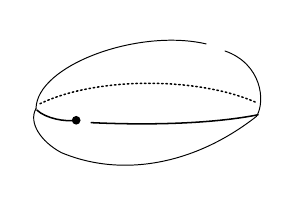
\begin{tikzpicture}[x=1cm,y=1cm,baseline=-0.35ex]
\draw[line width=0.35pt,line cap=round]
(-1.40,0) .. controls (-1.39,0.55) and (-0.10,1.02) .. (0.76,0.82);
\draw[line width=0.35pt,line cap=round]
(1.00,0.73) .. controls (1.46,0.57) and (1.52,0.10) .. (1.40,-0.10)
.. controls (0.61,-0.72) and (-0.32,-0.88) .. (-1.08,-0.56)
.. controls (-1.34,-0.42) and (-1.50,-0.18) .. (-1.40,0);
\draw[densely dotted,line width=0.55pt,line cap=round]
(-1.35,0.06) .. controls (-0.62,0.41) and (0.68,0.40) .. (1.41,0.07);
\draw[line width=0.55pt,line cap=round]
(-1.39,-0.02) .. controls (-1.27,-0.13) and (-1.03,-0.17) .. (-0.90,-0.15);
\fill (-0.89,-0.15) circle[radius=0.055];
\draw[line width=0.55pt,line cap=round]
(-0.70,-0.18) .. controls (0.17,-0.22) and (0.91,-0.18) .. (1.42,-0.08);
\end{tikzpicture}}
\unsure{formé|formée} d'un sommet, \unsure{sur} une arête (équateur) délimitant deux faces qui sont des monogones.

Le cas b) est le rev. cyclique d'ordre $3$ :
ramifié seulement en $0$ et en $\infty$ (en $1$ l'indice de ramification doit être diviseur de $2$ et de $3$,
donc est $1$) donc carte régulière sphérique de

\scanpage{573}
\mspage{291}

type $(3,3)$, avec des arêtes qui sont des boucles
\deleted{\illegible{1}}\inserted{repliées}

(76) \figure{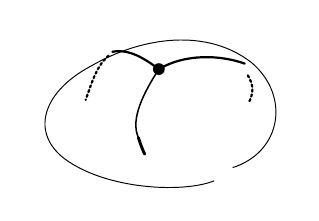
\begin{tikzpicture}[x=1cm,y=1cm,baseline=-0.35ex]
\draw[line width=0.35pt,line cap=round]
(0.89,-0.66) .. controls (1.51,-0.46) and (1.62,0.25) .. (1.13,0.67)
.. controls (0.57,1.11) and (-0.25,1.01) .. (-0.91,0.63)
.. controls (-1.57,0.28) and (-1.71,-0.29) .. (-1.14,-0.62)
.. controls (-0.61,-0.94) and (0.27,-0.98) .. (0.65,-0.83);
\draw[line width=0.8pt,line cap=round]
(-0.05,0.59) .. controls (-0.23,0.72) and (-0.42,0.85) .. (-0.64,0.81);
\draw[densely dotted,line width=0.8pt,line cap=round]
(-0.69,0.76) .. controls (-0.86,0.61) and (-0.91,0.38) .. (-0.98,0.20);
\draw[line width=0.8pt,line cap=round]
(-0.05,0.59) .. controls (0.29,0.79) and (0.73,0.77) .. (1.04,0.66);
\draw[densely dotted,line width=0.8pt,line cap=round]
(1.08,0.51) .. controls (1.16,0.38) and (1.15,0.28) .. (1.09,0.16);
\draw[line width=0.55pt,line cap=round]
(-0.05,0.59) .. controls (-0.23,0.31) and (-0.42,-0.04) .. (-0.31,-0.28);
\draw[line width=1.05pt,line cap=round]
(-0.31,-0.28) .. controls (-0.29,-0.35) and (-0.25,-0.45) .. (-0.23,-0.49);
\fill (-0.05,0.59) circle[radius=0.075];
\end{tikzpicture}}
: $1$ seul sommet,
trois arêtes repliées qui en sortent, une face
triangulaires. [Ces variétés modulaires sont
trop proches de $\widetilde M_{1,1}$ -- avec un groupe
d'autom (quotient de $\Gamma'_\infty=\mathrm{Sl}(2,\unsure{Z|\mathbb Z})$) trop petit,
pour pouvoir être rigidifiantes (il faudrait
que le groupe de Galois-Poincaré du rev.
soit multiple de $12$\inserted{(mult. de $4$ et de $6$ ?!)}, pour que \deleted{\illegible{1}} la courbe modulaire ait une chance d'être rigidifiante. Ces
cas semblent donc nettement moins intéressants.

Il y aurait lieu par ailleurs, dans chacun des
trois cas restants de (75) (mis à part donc le
premier cas, qui correspond à $M_{1,1}[2]'$ et est
à peu près compris), d'expliciter la relation
entre les points des courbes rationnelles
correspondantes, et entre \inserted{courbes elliptiques à} rigidifications de
Jacobi, d'échelon respectivement $3,4,5$. Et il y
a sûrement des choses précises dans Klein,
mais on aimerait faire des choses un peu
plus fines, qui soient valables simultanément
en \unsure{toutes caractéristiques|toute caractéristique} i.e. sur des schémas
de base généraux. Ce souci semble intimement lié à la question des opérations de
$\Gamma_{\mathbb Q}$ sur les classes d'isomorphie des cartes, et

\scanpage{574}

plus particulièrement des cartes sphériques
régulières. C'est assez extraordinaire que
Jean Malgoire, depuis trois ans que la
question est là, n'y ait pas encore touché
-- Dieu sait qu'elle est juteuse !

Complément sur le rapport anharmonique.

Soient $x_1,x_2,x_3,x_4$ des \deleted{variables, \unsure{en|ou} $\infty$}\inserted{sections \inserted{\unsure{partout}} distinctes} de
$\mathbb P^1_S$, on veut construire la section \unsure{correspondante} $\lambda$
de $\unsure{U|\mathbb U}_{0,3}=\mathbb P^1_S-\{0,1,\infty\}_S$.
Soient $a,b,c,d$ sections
(locales) de $\mathcal O_S$, \inserted{avec \deleted{\illegible{1}} $ad-bc$ inversible,} telles que
\[
u=u_{a,b,c,d}:\quad z\longmapsto\frac{az+b}{cz+d}
\tag{77}
\]
transforme $(x_1,x_2,x_3)$ en $(0,1,\infty)$ -- on
aura donc
\[
\lambda=u(x_4).
\tag{78}
\]
Les conditions sur \unsure{$\xi$|\deleted{\illegible{1}}} $(a,b,c,d)$ pour $ux_1=0$ etc sont
\[
\left\{\begin{aligned}
ax_1+b&=0\\
ax_2+b&=cx_2+d\\
cx_3+d&=0
\end{aligned}\right.
\]
qui donnent, si p. ex. $a$ est inversible (sinon, on
peut supposer $\unsure{c}$ inversible\ldots) en résolvant en $b,c,d$
\[
\left\{\begin{aligned}
b&=-ax_1\\
cx_2+d&=a(x_2-x_1)\\
cx_3+d&=0
\end{aligned}\right.
\qquad\left|\begin{aligned}
c&=a\frac{x_2-x_1}{x_2-x_3}\\
d&=-a\frac{x_2-x_1}{x_2-x_3}x_3
\end{aligned}\right.
\]
d'où
\[
\lambda=\frac{ax_4+b}{cx_4+d}
=\frac{a(x_4-x_1)}{a\frac{x_2-x_1}{x_2-x_3}x_4-a\frac{x_2-x_1}{x_2-x_3}x_3}
=\frac{(x_4-x_1)(x_2-x_3)}{(x_2-x_1)(x_4-x_3)}
\]

\scanpage{575}
\mspage{292}

\[
\lambda(x_1,x_2,x_3,x_4)=\frac{(x_4-x_1)(x_2-x_3)}{(x_2-x_1)(x_4-x_3)}
\tag{79}
\]

En tant que fonction rationnelle en $x_1,x_2,x_3,x_4$,
(à coeff. dans un anneau intègre fixé) elle
est caractérisé par les deux propriétés : a) invariance \unsure{p.r.} à une (même) transformation
homographique sur les variables, \inserted{$x_1,x_2,x_3,x_4$,} \deleted{et}
\[
f(ux_1,ux_2,ux_3,ux_4)=f(x_1,x_2,x_3,x_4),
\]
\inserted{et} b)
\[
f(0,1,\infty,x_4)=x_4
\]
(avec un grain de sel pour donner un
sens au premier \unsure{mb.} On a de plus
c) une propriété remarquable de symétrie,
qu'on \deleted{\illegible{1}} explicite en définissant un hom
de $\mathfrak S_4$ dans le groupe homographique
(\unsure{moralement|normalement}, $\mathrm{GP}(1)$)
\deleted{\illegible{1}}
\diagram{
\begin{tikzcd}[ampersand replacement=\&,column sep=large,row sep=large]
\mathfrak S_4 \arrow[rr,"\sigma\mapsto\varphi_\sigma"] \arrow[dr,"\text{épi}","\substack{\text{\unsure{se factorisant}}\\\text{par}}"'] \&\& \mathrm{GP}(1) \\
\& \mathfrak S_3 \arrow[ur] \&
\end{tikzcd}
}
de telle façon qu'on ait
\[
\lambda(x_{\sigma^{-1}1},x_{\sigma^{-1}2},x_{\sigma^{-1}3},x_{\sigma^{-1}4})
=\varphi_\sigma(\lambda(x_1,x_2,x_3,x_4))
\tag{80}
\]
\ldots
